
\section{shallow ice sheets}

\begin{frame}{slow, non-Newtonian, some basal slip, and shallow}

\begin{itemize}
\item ice sheets have four outstanding properties \emph{as fluids}:
  \begin{enumerate}
  \item slow
  \item non-Newtonian
  \item contact slip (sometimes)
  \item shallow
  \end{enumerate}
\end{itemize}
\end{frame}


\begin{frame}{regarding ``shallow''}

\begin{itemize}
\item below in \alert{red} is a no-vertical-exaggeration cross section of Greenland at $71^\circ$
\small
  \begin{itemize}
  \item[$\circ$] green and blue: standard vertically-exaggerated cross section
  \end{itemize}
  \begin{center}
    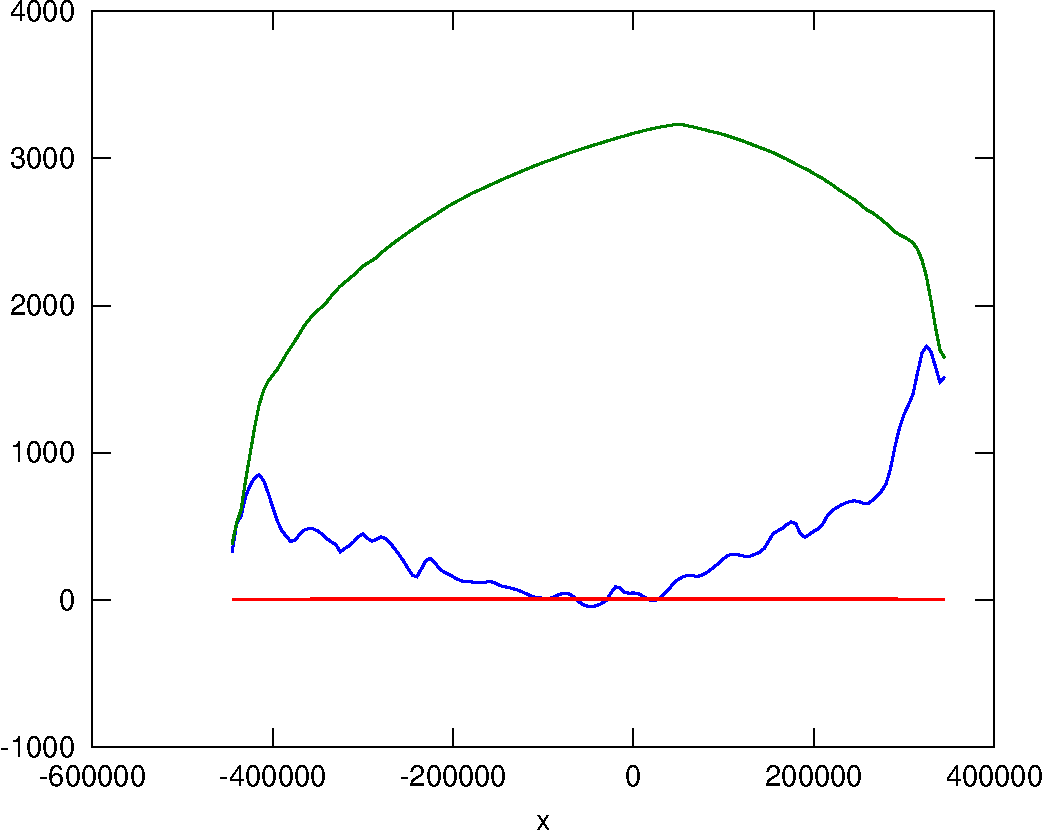
\includegraphics[width=0.6\textwidth]{green_transect}
  \end{center}
\item you can scale Stokes equation using smallness of $\eps = [H]/[L]$, where $[H]$ is a typical thickness of an ice sheet and $[L]$ is a typical horizontal dimension, \dots
\end{itemize}
\end{frame}


\subsection{shallow ice approx (SIA)}

\begin{frame}{non-sliding, isothermal shallow ice approximation = (SIA)}

a model which applies to
\begin{itemize}
\item shallow grounded ice sheets
\item on not-too-rough bed topography,
\item whose flow is not dominated by sliding and/or liquid water at the base or margin
\end{itemize}

\begin{center}
  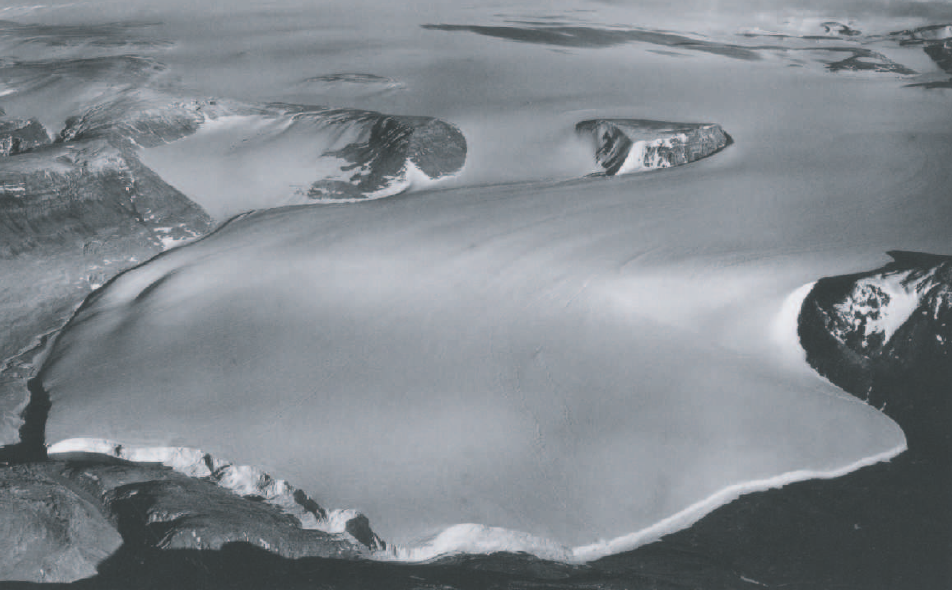
\includegraphics[width=0.65\textwidth]{polaris}

\tiny ``Polaris Glacier,'' northwest Greenland, photo 122, Post \& LaChapelle (2000)
\end{center}

\end{frame}


\begin{frame}{SIA velocity equation}

\begin{itemize}
\item \small here we ``derive'' the SIA by the simple slogan:\normalsize

\begin{center}
\emph{the SIA uses the formulas from slab-on-a-slope}
\end{center}
\item shear stress approximation:
	$$(\tau_{13},\tau_{23}) \approx - \rho g (h-z) \nabla h$$
\item let $\mathbf{U} = (u,v)$, the horizontal velocity
\item we further approximate
\begin{align*}
\mathbf{U}_z &\approx 2 A |(\tau_{13},\tau_{23})|^{n-1} (\tau_{13},\tau_{23}) \\
     &= - 2 A (\rho g)^n (h-z)^n |\nabla h|^{n-1} \nabla h
\end{align*}
\item by integrating vertically, in the non-sliding case,
    $$\mathbf{U} = - \frac{2 A (\rho g)^n}{n+1} \left[H^{n+1} - (h-z)^{n+1}\right] |\nabla h|^{n-1} \nabla h$$
\item but mass continuity remains, $H_t = M - \left(\overline{\mathbf{U}} H\right)_x$
\end{itemize}
\end{frame}


\begin{frame}{SIA thickness equation}

\begin{itemize}
\item combine last two equations on last slide
\item get the non-sliding, isothermal shallow ice approximation for thickness changes:
\begin{empheq}[box=\fbox]{equation*}
H_t = M + \Div \left(\Gamma H^{n+2} |\grad h|^{n-1} \grad h \right)
\end{empheq}

\vspace{-2mm}
  \begin{itemize}
  \item[$\circ$] where $H$ is ice thickness, $h$ is ice surface elevation, $b$ is bed elevation ($h=H+b$)
  \item[$\circ$] $M$ combines surface and basal mass (im)balance:

     accumulation if $M>0$, ablation if $M<0$
  \item[$\circ$] $n$ is the exponent in the Glen flow law
  \item[$\circ$] $\Gamma = 2 A (\rho g)^n / (n+2)$ is a positive constant
  \end{itemize}
\end{itemize}
\end{frame}


\begin{frame}{SIA thickness equation 2}

\begin{itemize}
\item numerically solve this equation
\begin{empheq}[box=\fbox]{equation}
H_t = M + \Div \left(\Gamma H^{n+2} |\grad h|^{n-1} \grad h \right) \label{sia}
\end{empheq}
and you've got a usable model for \dots \emph{the Barnes ice cap} (Mahaffy, 1976)
\end{itemize} 
\medskip

\begin{columns}
\begin{column}{0.5\textwidth}
\noindent good questions:
\begin{enumerate}
\item where does equation (1) come from?
\item how to solve it numerically?
\item how to \emph{think} about it?
\end{enumerate}  
\end{column}

\begin{column}{0.5\textwidth}
\begin{center}
  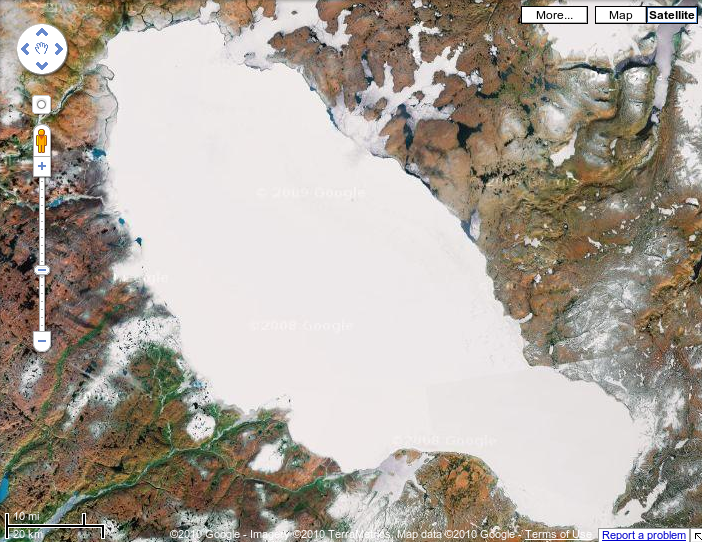
\includegraphics[width=0.8\textwidth]{barnes}
\end{center}
\end{column}
\end{columns}
\end{frame}


\subsection{analogy w heat equation}

\begin{frame}{heat equation}

\small
\begin{columns}
\begin{column}{0.6\textwidth}
\begin{itemize}
\item for understanding the SIA, recall the heat equation describing conduction
\item here's one quick way to derive it \dots
\item Newton's law of cooling for each segment of the rod:
\begin{align*}
\frac{dT_j}{dt} &= - C \left(T_j - \frac{1}{2} (T_{j-1} + T_{j+1}) \right) \\
	&= \frac{C}{2} \left(T_{j-1} - 2 T_j + T_{j+1}\right) 
\end{align*}
\item the limit as segments shrink $\Delta x\to 0$:
	$$T_t = D T_{xx}$$
\item $D=$ diffusivity, with units $\text{m}^2\,\text{s}^{-1}$
\item $T_{xx}>0 \implies T(t)$ decreases
\item $T_{xx}<0 \implies T(t)$ increases
\item so $T(x)$ becomes smoother with time
\end{itemize}
\end{column}

\begin{column}{0.4\textwidth}
\hfill
%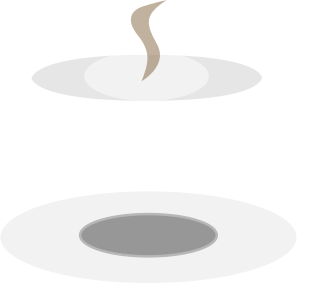
\includegraphics[width=0.5\textwidth]{coffee}
\vspace{0.3in}
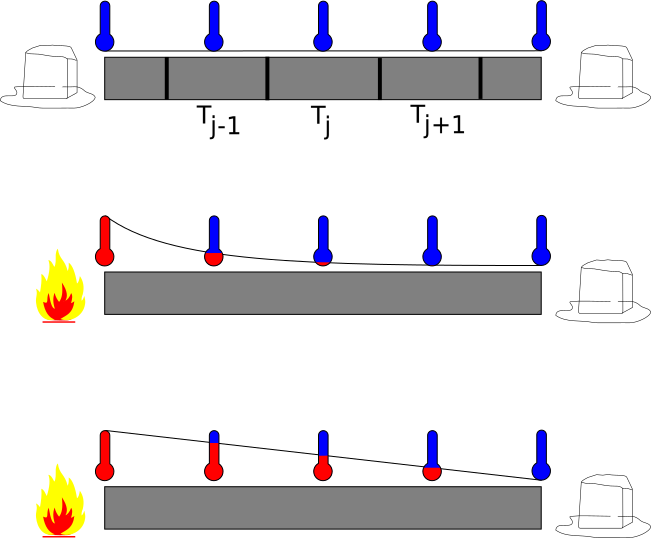
\includegraphics[width=1.0\textwidth]{heatconduction}
\end{column}
\end{columns}
\end{frame}


\begin{frame}{more complete heat equation}

\small
\begin{columns}
\begin{column}{0.6\textwidth}
\begin{itemize}
\item $T(t,x,y)$ is temperature in a 2D object at position $x,y$ and time $t$
\item Fourier rewrote Newton's law as a rule for heat flux: $\mathbf{q} = - k \grad T$
\item allow an additional heat source $f$
\item coefficients: $\rho$ is density, $c$ is specific heat, $k$ is conductivity
  \begin{itemize}
  \item[$\circ$] let's assume $\rho$, $c$ are constant
  \end{itemize}
\item by conservation of energy:
	$$\rho c T_t = f + \Div (k \grad T)$$
\end{itemize}
\end{column}
\begin{column}{0.4\textwidth}
\animategraphics[autoplay,loop,height=2.5cm]{4}{anim/heatmelt}{0}{16}
\end{column}
\end{columns}

\begin{itemize}
\item define the diffusivity $D=k/(\rho c)$ and also $F := f/(\rho c)$
\item for 2D object (e.g.~a plate), the heat equation:
\begin{equation}
T_t = F + \Div (D\, \grad T) \label{heat}
\end{equation}
\item the temperature $T$ solves a \emph{diffusive, time-evolving partial differential equation (PDE)} \dots just like thickness $H$ in SIA
\end{itemize}
\end{frame}


\begin{frame}{analogy: SIA versus heat equation}

\begin{itemize}
\item side-by-side comparison:
\begin{center}
\begin{tabular}{cc}
\scriptsize SIA:\, $H(t,x,y)$ is ice thickness & \scriptsize heat: $T(t,x,y)$ is temperature \normalsize \\
	\boxed{H_t = M + \Div \left({\color{red}\Gamma H^{n+2} |\grad h|^{n-1}}\, \grad h \right)}  &  \boxed{T_t = F + \Div (D\, \grad T)}
\end{tabular}
\end{center}

\medskip
\item we identify the diffusivity in the SIA:
	$$D = {\color{red}\Gamma H^{n+2} |\grad h|^{n-1}}$$
\item \emph{non-sliding shallow ice flow \alert{diffuses} the ice sheet}
\item some issues with this analogy:
  \begin{itemize}
  \item[$\circ$]  $D$ depends on solution $H(t,x,y)$
  \item[$\circ$]  $D\to 0$ at margin, where $H\to 0$
  \item[$\circ$]  $D\to 0$ at divides/domes, where $|\grad h|\to 0$
  \end{itemize}
\end{itemize}
\end{frame}


\subsection{finite difference numerics}

\begin{frame}{basic ideas of finite differences}

\begin{itemize}
\item numerical schemes for heat equation are good start for SIA
\item for differentiable $f(x)$ and any $\Delta$, \emph{Taylor's theorem} says
	$$f(x+\Delta) = f(x) + f'(x) \Delta + \frac{1}{2} f''(x) \Delta^2 + \frac{1}{3!} f'''(x) \Delta^3 + \dots$$
\normalsize
\item you can replace ``$\Delta$'' by its multiples, e.g.:
\small
\begin{align*}
f(x-\Delta) &= f(x) - f'(x) \Delta + \frac{1}{2} f''(x) \Delta^2 - \frac{1}{3!} f'''(x) \Delta^3 + \dots \\
f(x+2\Delta) &= f(x) + 2 f'(x) \Delta + 2 f''(x) \Delta^2 + \frac{4}{3} f'''(x) \Delta^3 + \dots
\end{align*}
\normalsize
\item basic finite difference idea:
\begin{quote}
\emph{combine expressions like these to give approximations of derivatives from values of $f(x)$ on a grid}
\end{quote}
\end{itemize}
\end{frame}


\begin{frame}{finite differences for partial derivatives}

\begin{itemize}
\item we want partial derivative expressions, for example with some function $u=u(t,x)$:
\small
\begin{align*}
u_t(t,x) &= \frac{u(t+\Delta t,x) - u(t,x)}{\Delta t} + O(\Delta t), \\
u_t(t,x) &= \frac{u(t+\Delta t,x) - u(t-\Delta t,x)}{2\Delta t} + O(\Delta t^2), \\
u_x(t,x) &= \frac{u(t,x+\Delta x) - u(t,x)}{\Delta x} + O(\Delta x), \\
u_{xx}(t,x) &= \frac{u(t,x+\Delta x) - 2 u(t,x) + u(t,x-\Delta x)}{\Delta x^2} + O(\Delta x^2)
\end{align*}
\normalsize
\item sometimes we want a derivative in-between grid points:
\small
	$$u_x(t,x+(\Delta x/2)) = \frac{u(t,x+\Delta x) - u(t,x)}{\Delta x} + O(\Delta x^2)$$
\normalsize
\item ``$+O(\Delta^2)$'' is better than ``$+O(\Delta)$'' if $\Delta$ is a small number
\end{itemize}
\end{frame}


\begin{frame}{explicit scheme for heat equation}
\label{slide:explicit}

\begin{itemize}
\item recall 1D heat equation $T_t = D T_{xx}$
\item an \emph{explicit} scheme:
\small
	$$\frac{T(t+\Delta t,x) - T(t,x)}{\Delta t} = D\,\frac{T(t,x+\Delta x) - 2 T(t,x) + T(t,x-\Delta x)}{\Delta x^2}$$
\normalsize
\item the difference between the equation $T_t = D T_{xx}$ and the scheme is $O(\Delta t,\Delta x^2)$
\item notation: $(t_n,x_j)$ and $T_j^n \approx T(t_n,x_j)$
\item let $\mu = D \Delta t / (\Delta x)^2$, so
\small
	$$T_j^{n+1} = \mu T_{j+1}^n + (1 - 2 \mu) T_j^n + \mu T_{j-1}^n$$
\normalsize
\end{itemize}
\begin{columns}
\begin{column}{0.55\textwidth}
\begin{itemize}
\item scheme has stencil at right \large $\to$ \normalsize
\end{itemize}
\end{column}
\begin{column}{0.45\textwidth}
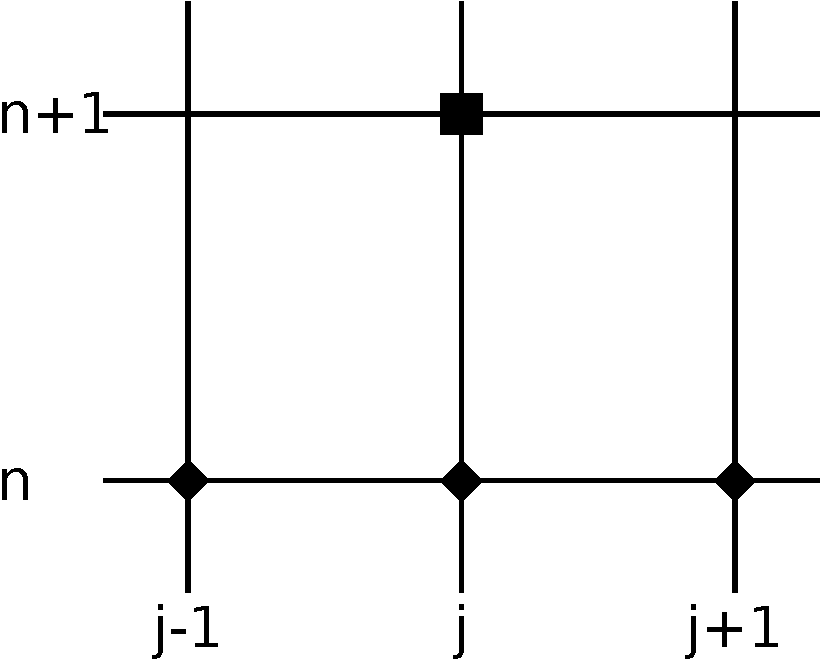
\includegraphics[width=0.7\textwidth]{expstencil}
\end{column}
\end{columns}
\end{frame}


\begin{frame}{explicit scheme in two space dimensions}

\begin{itemize}
\item recall heat equation in 2D: $T_t = D(T_{xx} + T_{yy})$
\item in two spatial variables we write $T_{jk}^n \approx T(t_n,x_j,y_k)$
\item so the 2D explicit scheme is
\small
	$$\frac{T_{jk}^{n+1} - T_{jk}^n}{\Delta t} = D\,\left(\frac{T_{j+1,k}^n - 2 T_{jk}^n + T_{j-1,k}^n}{\Delta x^2} + \frac{T_{j,k+1}^n - 2 T_{jk}^n + T_{j,k-1}^n}{\Delta y^2}\right)$$
\end{itemize}

\bigskip
\begin{center}
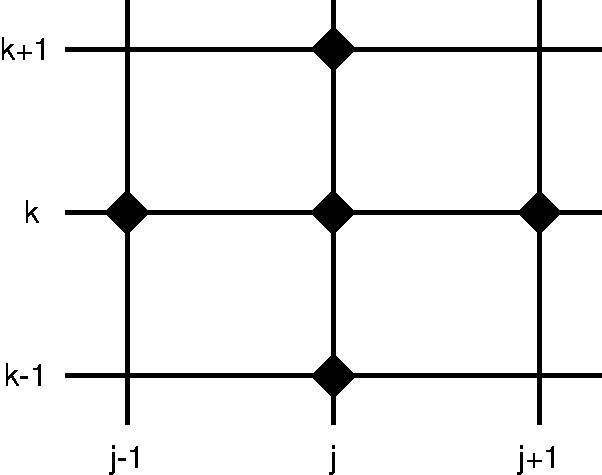
\includegraphics[width=0.35\textwidth]{exp2dstencil}
\end{center}
\end{frame}


\begin{frame}{implementation}
\label{slide:heatmatlab}

\minput{heat}

\small
\begin{itemize}
\item solves $T_t = D(T_{xx} + T_{yy})$ on square $-1 < x < 1$, $-1 < y < 1$
\item uses gaussian initial condition: $T(0,x,y) = e^{-30 r^2}$
\item uses ``colon notation'' to remove loops over spatial variables
\item \texttt{>>  heat(1.0,30,30,0.001,20)}

approximates $T$ on $30\times 30$ spatial grid, with $D=1$ and $N=20$ steps of $\Delta t = 0.001$
\end{itemize}
\end{frame}


\begin{frame}{the look of success}

\begin{itemize}
\item solving $T_t = T_{xx} + T_{yy}$ on $30\times 30$ grid
\end{itemize}

\bigskip
\begin{columns}
\begin{column}{0.5\textwidth}
initial condition $T(0,x,y)$

\phantom{foo}

\bigskip
\begin{center}
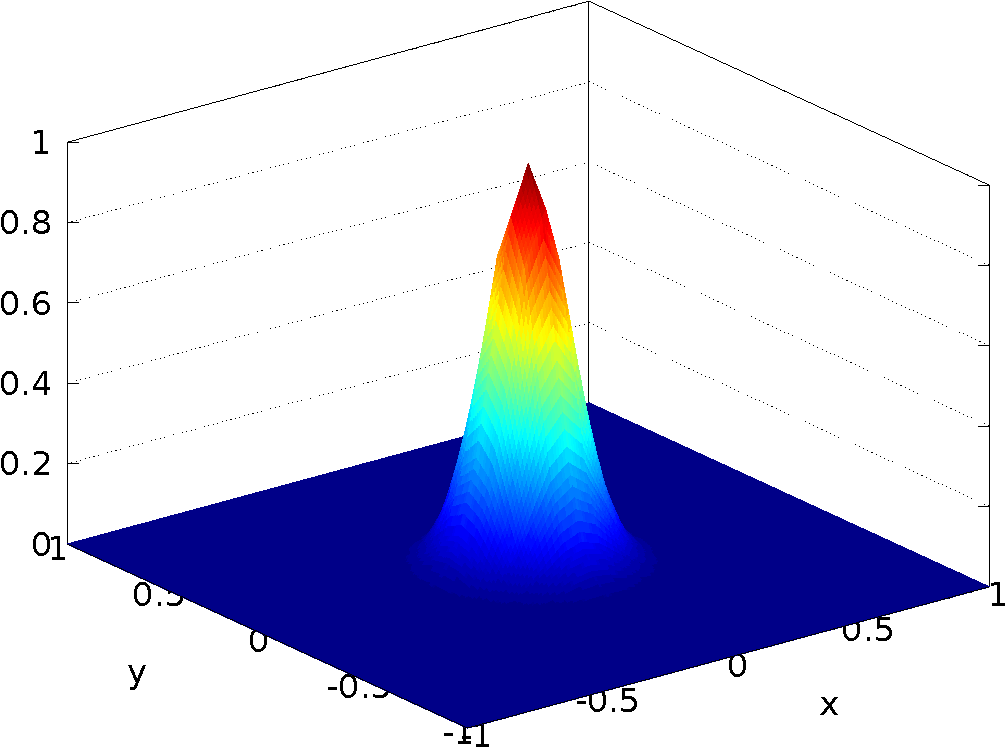
\includegraphics[width=1.0\textwidth]{initialheat}
\end{center}
\end{column}
\begin{column}{0.5\textwidth}
approximate solution $T(t,x,y)$ at $t=0.02$ with $\Delta t=0.001$ 

\bigskip
\begin{center}
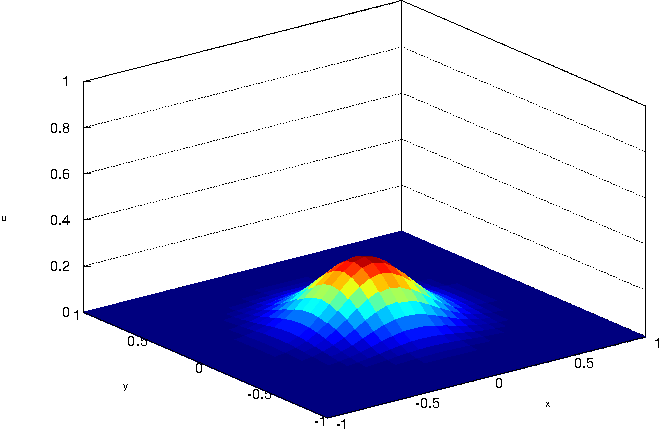
\includegraphics[width=1.0\textwidth]{finalheat}
\end{center}
\end{column}
\end{columns}
\end{frame}


\begin{frame}{the look of instability}

\begin{itemize}
\item figures below are from solving $T_t = T_{xx} + T_{yy}$ on the same space grid, but with slightly different time steps
\end{itemize}

\bigskip\bigskip
\begin{columns}
\begin{column}{0.5\textwidth}
\begin{center}
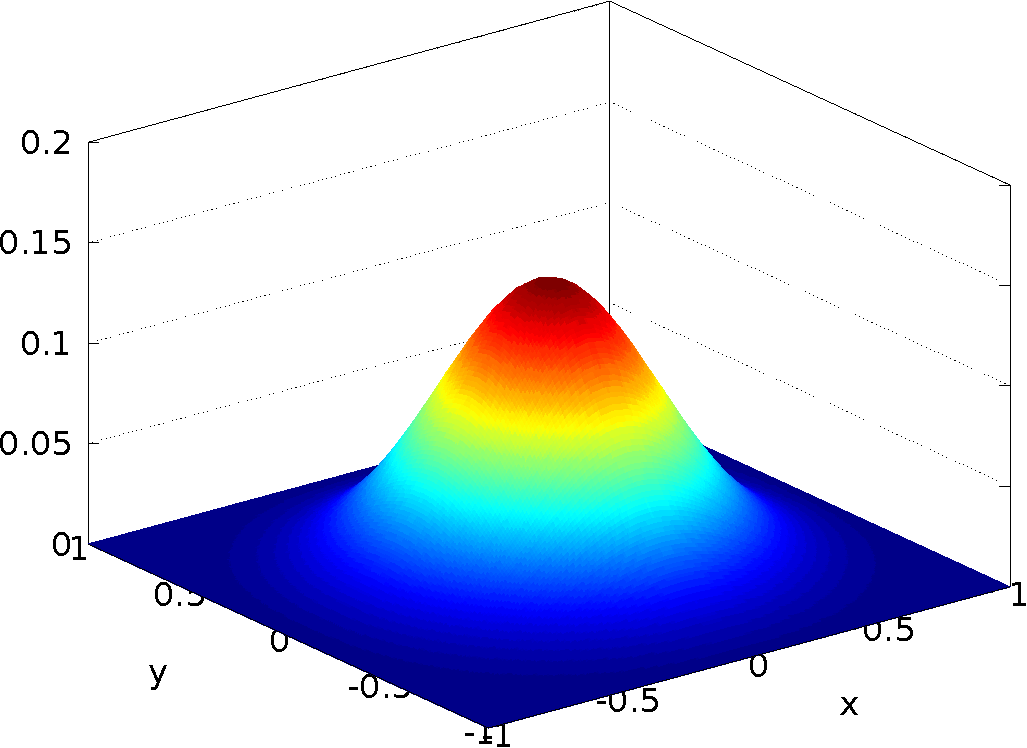
\includegraphics[width=1.0\textwidth]{stability}

$$\frac{D\Delta t}{\Delta x^2}= 0.2$$
\end{center}
\end{column}
\begin{column}{0.5\textwidth}
\begin{center}
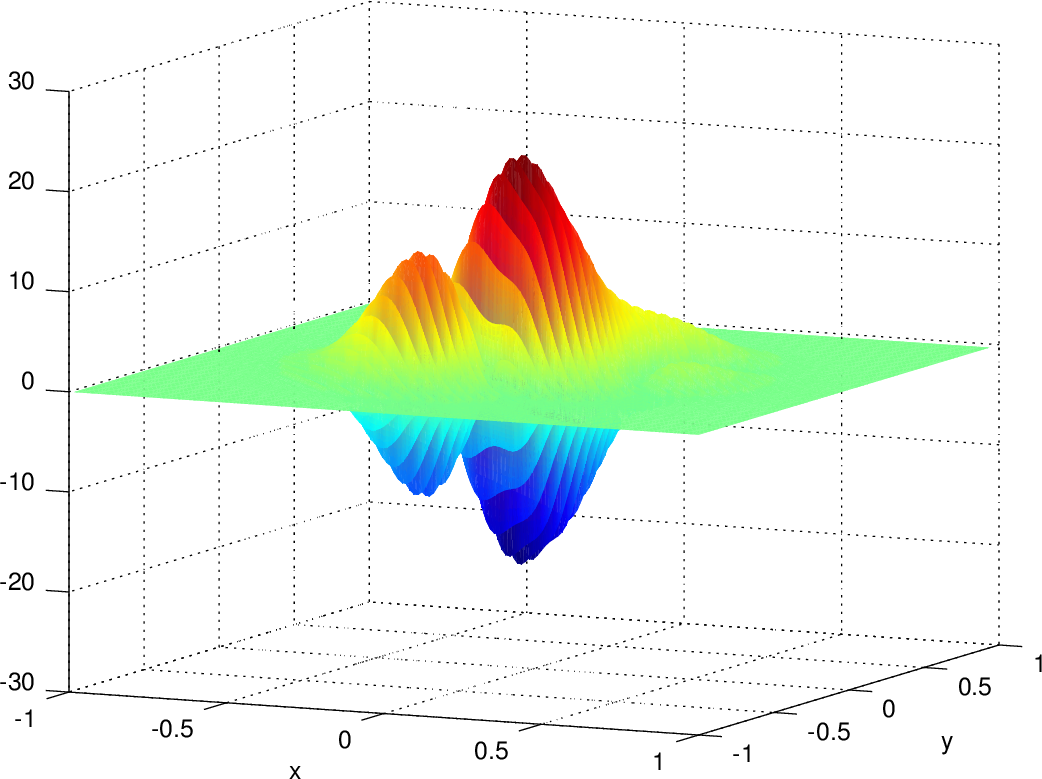
\includegraphics[width=1.0\textwidth]{instability}

$$\frac{D\Delta t}{\Delta x^2}= 0.4$$
\end{center}
\end{column}
\end{columns}
\end{frame}


\begin{frame}{avoid the instability}

\begin{itemize}
\item recall 1D explicit scheme has form 
	$$T_j^{n+1} = \mu T_{j+1}^n + (1 - 2 \mu) T_j^n + \mu T_{j-1}^n$$
\item thus the new value $T_j^{n+1}$ is an \emph{average} of the old values, \emph{if the middle coefficient is positive}:
	$$1 - 2 \mu \ge 0 \quad \iff \quad  \frac{D\Delta t}{\Delta x^2} \le \frac{1}{2} \quad \iff \quad \Delta t \le \frac{\Delta x^2}{2 D}$$
\item averaging is always stable because averaged wiggles are always smaller than the original wiggles
\item this condition is a sufficient \emph{stability criterion}
\item \emph{the result was unstable because the time step was too big}
\item in 2D case with $\Delta x= \Delta y$ the condition is
	$$\frac{D\Delta t}{\Delta x^2} \le \frac{1}{4}$$
\end{itemize}
\end{frame}


\begin{frame}{\textsl{adaptive} implementation: guaranteed stability}

\scriptsize
\minput{heatadapt}
\normalsize

\begin{itemize}
\item same as \texttt{heat.m} except

\begin{center}
\emph{choose time step from stability criterion}
\end{center}
\end{itemize}\end{frame}


\begin{frame}{alternative instability fix: implicitness}

\begin{itemize}
\item explicit scheme is only ``conditionally stable''
  \begin{itemize}
  \item[$\circ$] the adaptive implementation uses the condition
  \end{itemize}
\item there are \alert{implicit} methods which are stable for \emph{any} $\Delta t$
\item an implicit scheme for the heat equation is \emph{Crank-Nicolson}
  \begin{itemize}
  \item[$\circ$] it has smaller error too: $O(\Delta t^2,\Delta x^2)$
  \end{itemize}
\item \emph{but} you have to solve systems of equations at each time step
\item in nonlinear case you may end up spending much more programmer time to implement implicit methods
  \begin{itemize}
  \item[$\circ$] this can impose a big opportunity cost
  \end{itemize}
\vspace{5mm}

\item \small Donald Knuth has advice for ice sheet modelers: \begin{quote}
\emph{We should forget about small efficiencies \dots: premature optimization is the root of all evil}.
\end{quote}
\end{itemize}
\end{frame}


\begin{frame}{variable diffusivity}

\begin{itemize}
  \item recall the analogy: \qquad (SIA) $\leftrightarrow$ (heat eqn)
  \item the SIA has a diffusivity $D(x,y)$ which varies in space
  \item and it has both $H$ and $h=H+b$
  \item so consider a more general heat equation:
\begin{equation}
T_t = F + \Div \left(D\, \grad (T+b)\right) \tag{$\ast$}
\end{equation}
  \item the best explicit method for $(\ast)$ evaluates diffusivity $D$ at \alert{staggered} grid points:
  \scriptsize
\begin{align*}
\Div \left(D \grad X\right) &\approx \frac{D_{j+1/2,k}(X_{j+1,k} - X_{j,k}) - D_{j-1/2,k}(X_{j,k} - X_{j-1,k})}{\Delta x^2} \\
	&\qquad + \frac{D_{j,k+1/2}(X_{j,k+1} - X_{j,k}) - D_{j,k-1/2}(X_{j,k} - X_{j,k-1})}{\Delta y^2}
\end{align*}
\end{itemize}

\vspace{-0.15in}
\small
\begin{columns}
\begin{column}{0.55\textwidth}
\begin{itemize}
\item best = just as stable as previous
\item in stencil at right:
  \begin{itemize}
  \item[] diamonds: $X = T+b$
  \item[] triangles: $D$
  \end{itemize}
\end{itemize}
\end{column}
\begin{column}{0.45\textwidth}
\begin{center}
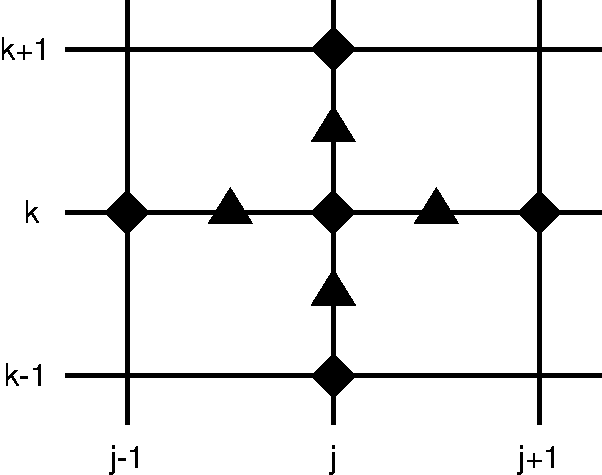
\includegraphics[width=0.6\textwidth]{diffstencil}
\end{center}
\end{column}
\end{columns}
\end{frame}


\begin{frame}
  \frametitle{general diffusion equation code}

\minputtiny{diffusion}

\small
\begin{itemize}
\item solves abstract diffusion equation $T_t = \Div \left(D \, \grad (T + b)\right)$
\item user supplies diffusivity $D$ on staggered grid
\end{itemize}
\end{frame}


\subsection{solutions}

\begin{frame}{exact solution of heat equation}

\begin{itemize}
\item before getting to ice flow, one more heat equation topic \dots
\vspace{5mm}

\item many \emph{exact} solutions to the heat equation are known
\item I'll show the ``Green's function''
\item \dots also known as ``heat kernel''
\item it starts at time $t=0$ with a ``delta function'' of heat at the origin $x=0$ and then it spreads out over time
\item we find it by a method which generalizes to the SIA
\end{itemize}
\end{frame}


\begin{frame}{Green's function of heat equation}

\begin{itemize}
\item the solution is ``self-similar'' over time
\item with time it changes shape by
  \begin{itemize}
  \item[$\circ$] shrinking the output (vertical) axis and
  \item[$\circ$] lengthening the input (horizontal) axis
  \end{itemize}
\item \dots but otherwise it is the same shape
\item the integral over $x$ is independent of time
\end{itemize}

\begin{center}
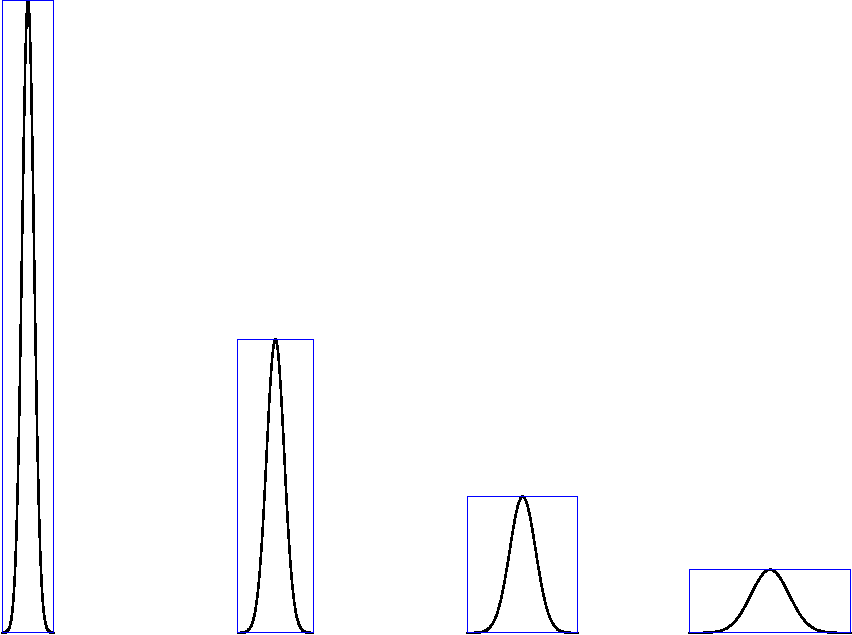
\includegraphics[width=0.5\textwidth]{heatscaling}

\emph{increasing time} \Large $\to$
\end{center}
\end{frame}


\begin{frame}{similarity solutions}

\begin{itemize}
\item Green's function of 1D heat equation ( $T_t=D T_{xx}$ ) is
	$$T(t,x) = C\, t^{-1/2} e^{-x^2/(4Dt)}$$
\item ``similarity'' variables for 1D heat equation are
	$$s \stackrel{\text{\emph{input scaling}}}{\phantom{\Big|}=\phantom{\Big|}} t^{-1/2} x, \qquad u(t,x) \stackrel{\text{\emph{output scaling}}}{\phantom{\Big|}=\phantom{\Big|}} t^{-1/2} \phi(s)$$
\end{itemize}
\begin{columns}
\begin{column}{0.6\textwidth}
\begin{itemize}
\item \emph{historical note}:  in 1905 Einstein saw that the average distance traveled by particles in thermal motion scales like $\sqrt{t}$, so $s = t^{-1/2}x$ is an invariant
\end{itemize}
\end{column}
\begin{column}{0.4\textwidth}
\begin{center}
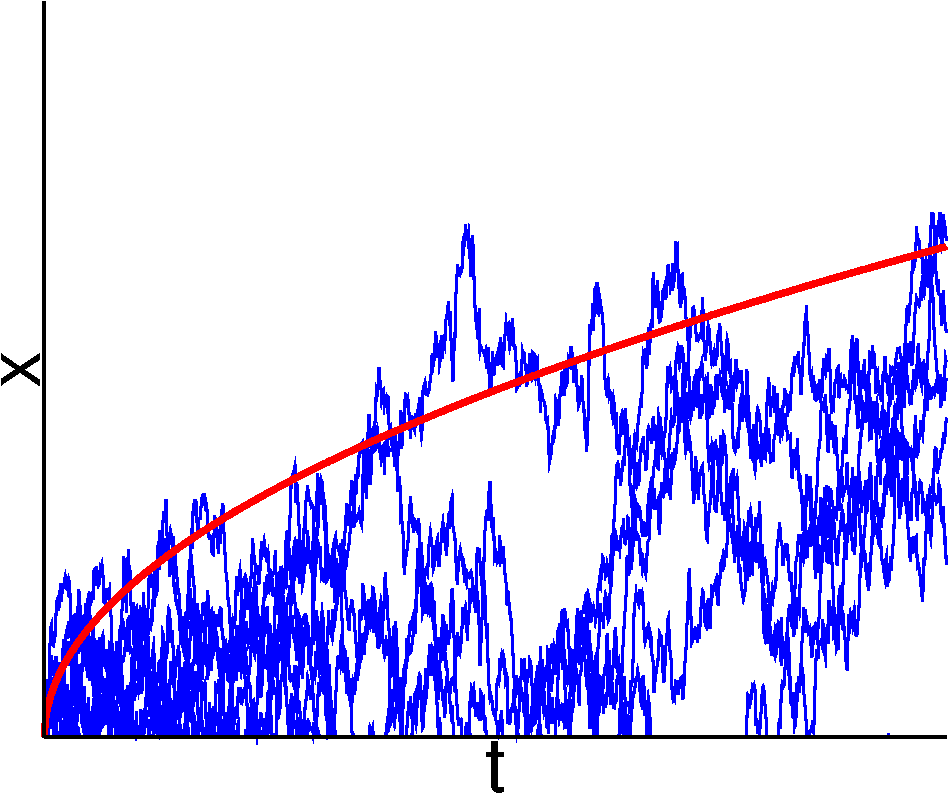
\includegraphics[width=1.0\textwidth]{brownian}
\end{center}
\end{column}
\end{columns}

\end{frame}


\subsection{solving the SIA}

\begin{frame}{similarity solution to SIA}

\begin{itemize}
\item jump forward to 1981
\item P.~Halfar found the similarity solution of the SIA in the case of flat bed and no surface mass balance
\item Halfar's 2D solution for Glen flow law with $n=3$ has scalings
	$$s \stackrel{\text{\emph{input scaling}}}{\phantom{\Big|}=\phantom{\Big|}} t^{-1/18} r, \qquad H(t,r) \stackrel{\text{\emph{output scaling}}}{\phantom{\Big|}=\phantom{\Big|}} t^{-1/9} \phi(s)$$
\item so: the nonlinear diffusion of the SIA quickly slows down the rate of change of the profile as the shape flattens out
\end{itemize}
\end{frame}


\begin{frame}{Halfar solution to the SIA: the movie}
\label{slide:plothalfar}

\animategraphics[autoplay,loop,height=7.0cm]{4}{anim/halfar}{0}{26}

\par
\scriptsize 
frames from $t=4$ months to $t = 10^6$ years, equal spaced in \emph{exponential} time
\end{frame}


\begin{frame}{Halfar solution to the SIA: the formula}

\begin{itemize}
\item for $n=3$ the solution formula is:
  $$H(t,r) = H_0 \left(\frac{t_0}{t}\right)^{1/9} \left[1 - \left(\left(\frac{t_0}{t}\right)^{1/18} \frac{r}{R_0}\right)^{4/3}\right]^{3/7}$$
\item the ``characteristic time'' is
  $$t_0 = \frac{1}{18 \Gamma} \left(\frac{7}{4}\right)^3 \frac{R_0^4}{H_0^{7}}$$
if $H_0$, $R_0$ are central height and ice cap radius at $t=t_0$
\item you choose $H_0$ and $R_0$ and then determine $t_0$
\item it is a simple formula to use for verification!
\end{itemize}
\end{frame}


\begin{frame}{is the Halfar solution \emph{good for any modelling}?}

\begin{itemize}
\item John Nye and others (2000) compared long-time consequences of different flow laws for the Mars polar caps
\item they evaluated $\text{CO}_2$ ice versus $\text{H}_2\text{O}$ ice parameters
\item \dots by comparing long-time behavior of the Halfar solutions
\item conclusions:
  \begin{quote}
  \dots none of the three possible [$\text{CO}_2$] flow laws will allow a 3000-m cap, the thickness suggested by stereogrammetry, to survive for $10^7$ years, indicating that the south polar ice cap is probably not composed of pure $\text{CO}_2$ ice \dots the south polar cap probably consists of water ice, with an unknown admixture of dust.
  \end{quote}
\end{itemize}

\end{frame}


\begin{frame}{on ``degenerate'' diffusivity}

\begin{itemize}
\item recall that the SIA is
\small
	$$H_t = M + \Div \left(D\, \grad h \right) \quad \text{where} \quad D = \Gamma H^{n+2} |\grad h|^{n-1}$$
\normalsize
\item thus the diffusivity ``degenerates'', $D \to 0$, when either $H\to 0$ or $\grad h \to 0$
\item summary:
\small
\begin{tabular}{l|c|c}
 & why $D\to 0$ & so what? \\ \hline
domes    & $\grad h \to 0$ & \begin{tabular}{c}
$H$ and $\grad h$ are continuous \\ but $\grad^2 h$ is singular
\end{tabular} \\ \hline
margins  & $H \to 0$       & \begin{tabular}{c}
$H$ is continuous \\ but $\grad h$ is singular
\end{tabular}
\end{tabular}
\normalsize
\item in terms of numerical error, margin is worse than dome
\item degenerate diffusion equations are automatically free boundary problems
\end{itemize}
\end{frame}


\begin{frame}
  \frametitle{computing diffusivity in SIA}

\begin{itemize}
\item for numerical stability we compute $D = \Gamma H^{n+2} |\grad h|^{n-1}$ on the staggered grid
\item various schemes proposed
\item all schemes involve
  \begin{itemize}
  \item[$\circ$] averaging $H$
  \item[$\circ$] differencing $h$
  \item[$\circ$] in a ``balanced'' way, for better accuracy,
  \end{itemize}
to get the diffusivity on staggered grid
\end{itemize}

\begin{columns}
\begin{column}{0.65\textwidth}
\begin{itemize}
\item Mahaffy's scheme has stencil \large $\to$ \normalsize
\end{itemize}
\end{column}

\begin{column}{0.35\textwidth}
  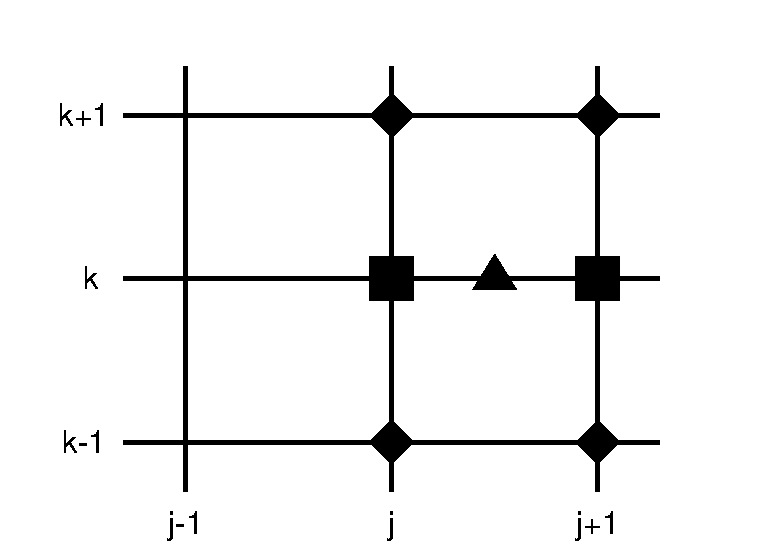
\includegraphics[width=1.0\textwidth]{mahaffystencil}
\end{column}
\end{columns}
\end{frame}


\begin{frame}
  \frametitle{SIA implementation: flat bed case}

\minputtiny{siaflat}

\end{frame}


\begin{frame}{verification of numerical ice flow codes}
\begin{itemize}
\item how do we make sure a numerical scheme is correct?

\vspace{5mm}
\item how do we make sure an \emph{implemented} numerical scheme is correct?
  \begin{itemize}
  \item[$\circ$] \emph{technique} 1: don't make any mistakes
  \item[$\circ$] \emph{technique} 2: compare your model with others, and hope that the outliers are the ones with errors
  \item[$\circ$] \emph{technique} 3: build-in a comparison to an exact solution, and actually measure the numerical error
  \end{itemize}

\vspace{5mm}
\item technique 3 is called \alert{verification}
\end{itemize}
\end{frame}


\begin{frame}{where to get exact solutions for ice flow models?}

\small
\begin{itemize}
  \item textbook: Greve and Blatter (2009)
  \item similarity solutions to SIA (Halfar 1983; Bueler et al 2005)
  \item manufactured solutions to thermo-coupled SIA (Bueler et al 2007)
  \item flowline and cross-flow SSA solutions (van der Veen, 1985; Schoof, 2006)
  \item flowline Blatter solutions (Glowinski and Rappaz 2003)
  \item flowline Stokes solutions for constant viscosity (Ladyzhenskaya 1963; Balise and Raymond 1985)
  \item manufactured solutions to the Stokes equations (Sargent and Fastook 2010; Jouvet and Rappaz 2011)
\end{itemize}
\end{frame}


\begin{frame}[fragile]
\frametitle{verifying SIA code vs Halfar}
\label{slide:verifysia}

\begin{columns}
\begin{column}{0.6\textwidth}
\scriptsize
\begin{verbatim}
octave:40> verifysia(20)
average abs error            = 22.310
maximum abs error            = 227.849
octave:41> verifysia(40)
average abs error            = 9.490
maximum abs error            = 241.470
octave:42> verifysia(80)
average abs error            = 2.800
maximum abs error            = 155.796
octave:43> verifysia(160)
average abs error            = 1.059
maximum abs error            = 109.466
\end{verbatim}
\normalsize

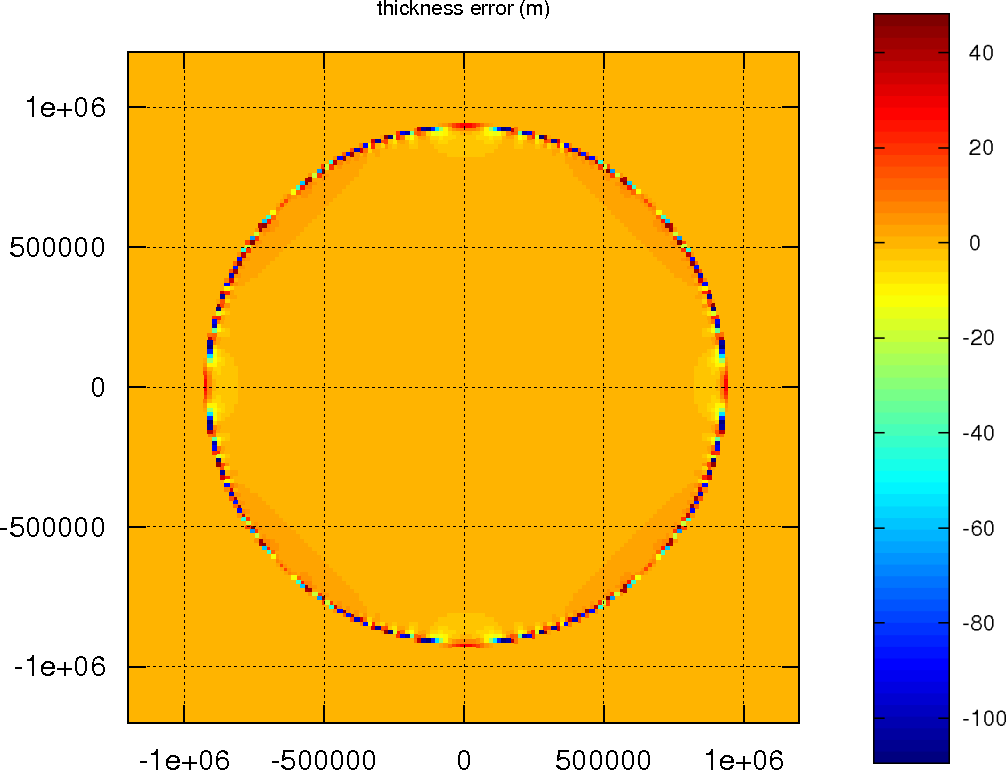
\includegraphics[width=0.8\textwidth]{siaerror}
\end{column}

\begin{column}{0.4\textwidth}
\small
\emph{Trust but verify.}
\medskip

\scriptsize
(Ronald Reagan)

\bigskip\bigskip\bigskip

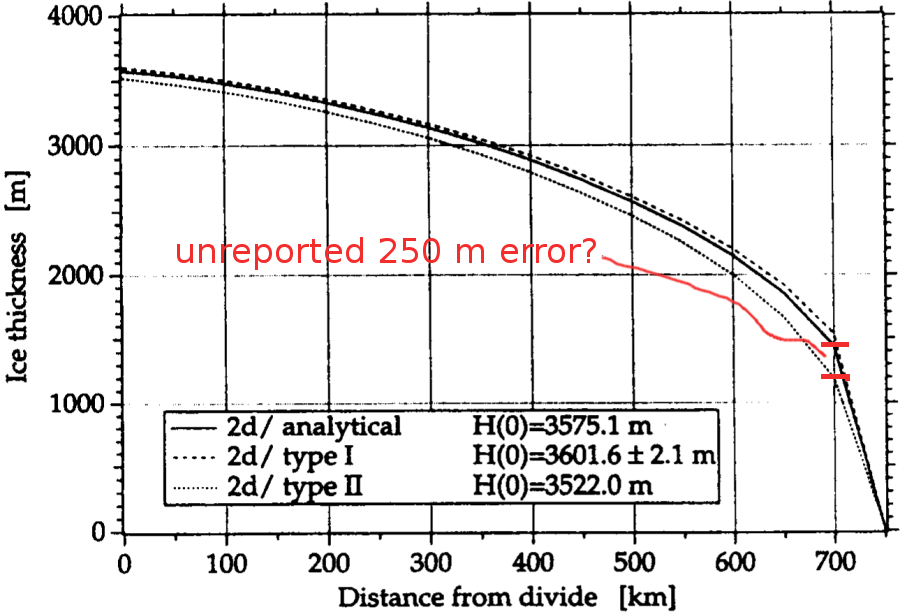
\includegraphics[width=1.0\textwidth]{eismintone}

\scriptsize \emph{figure 2 in Huybrechts et al.~(1996)}
\end{column}
\end{columns}
\end{frame}


\begin{frame}{demonstrate robustness}

see \texttt{roughice.m}, which calls \texttt{siaflat.m} after setting-up the nasty initial state at left:
\medskip

\begin{columns}
\begin{column}{0.5\textwidth}
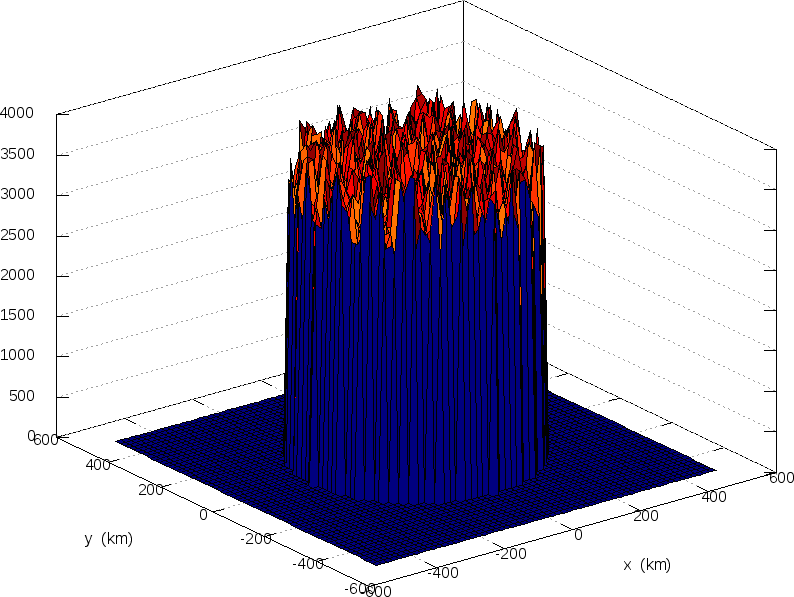
\includegraphics[width=1.0\textwidth]{roughinitial}
\end{column}
\begin{column}{0.5\textwidth}
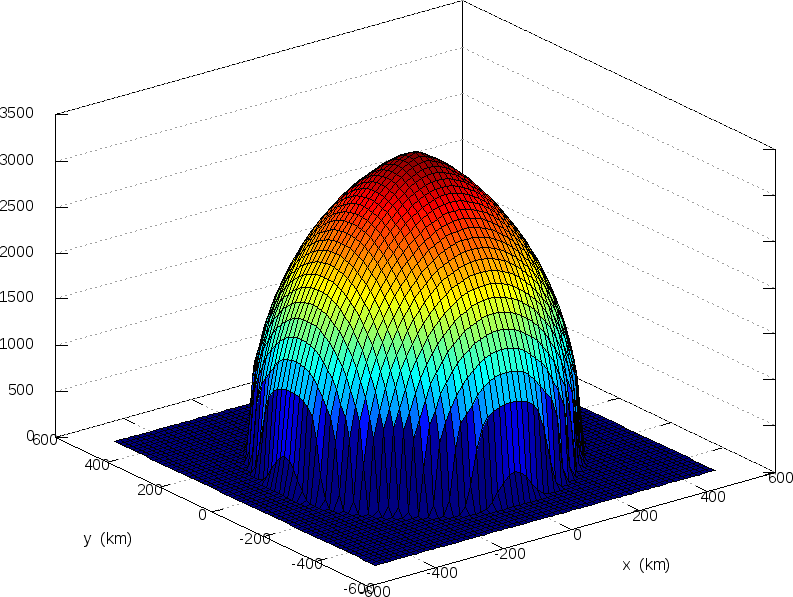
\includegraphics[width=1.0\textwidth]{roughfinal}
\end{column}
\end{columns}

\begin{center}
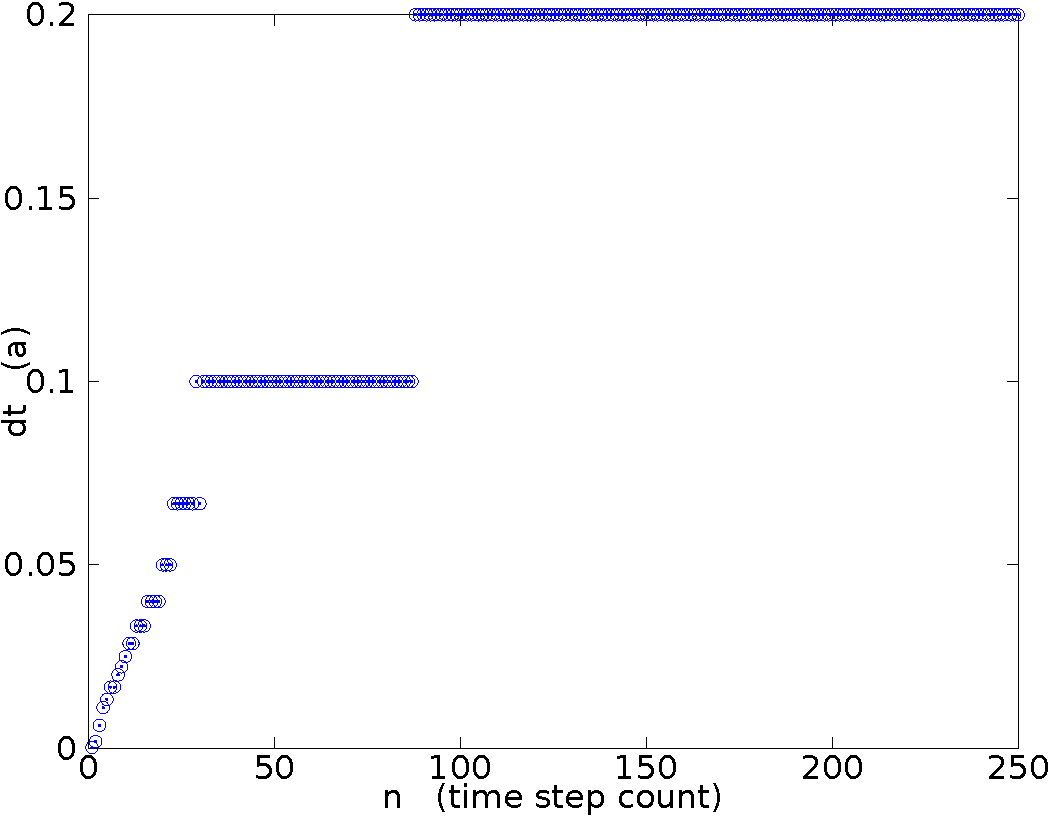
\includegraphics[width=0.4\textwidth]{roughtimesteps}
\end{center}
\end{frame}


\begin{frame}{model the Antarctic ice sheet}

\normalsize
\begin{itemize}
\item with careful-but-small modifications of \texttt{siaflat.m}, which make a good exercise:
  \begin{itemize}
  \item[$\circ$] observed accumulation as surface mass balance,
  \item[$\circ$] allow non-flat bed (so $H\ne h$),
  \item[$\circ$] differentiate the surface correctly where floating, and
  \item[$\circ$] calve at current calving front location
  \end{itemize}
here are results from this \emph{toy} Antarctic flow model
\item a 2000 model year run on a $\Delta x=50$ km grid; runtime a few seconds
\end{itemize}

\bigskip

\begin{columns}
\begin{column}{0.4\textwidth}
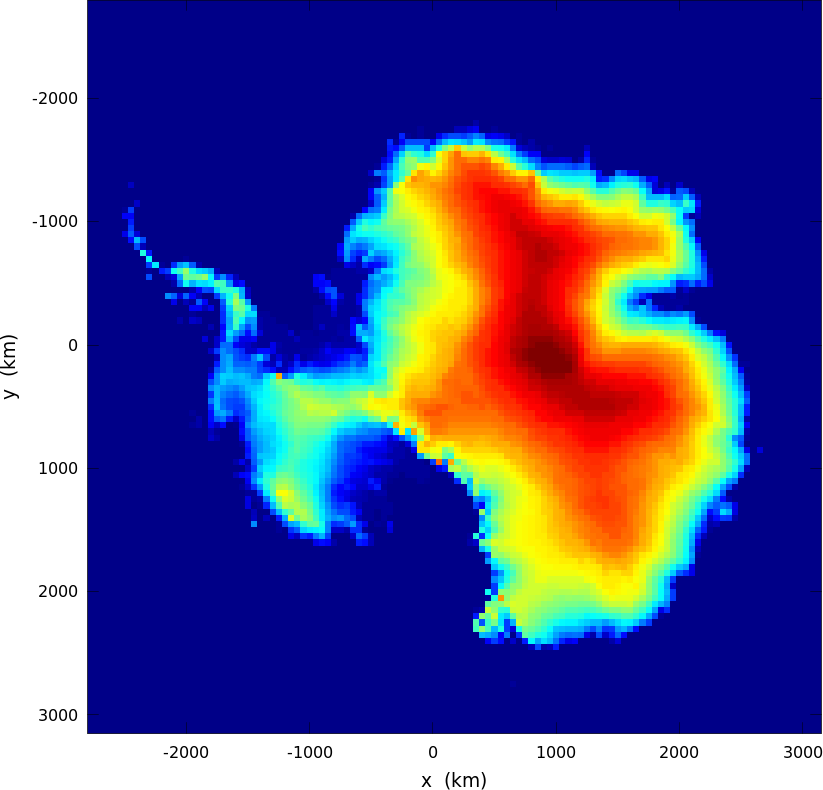
\includegraphics[height=1.75in]{antinitial}
\end{column}
\begin{column}{0.55\textwidth}
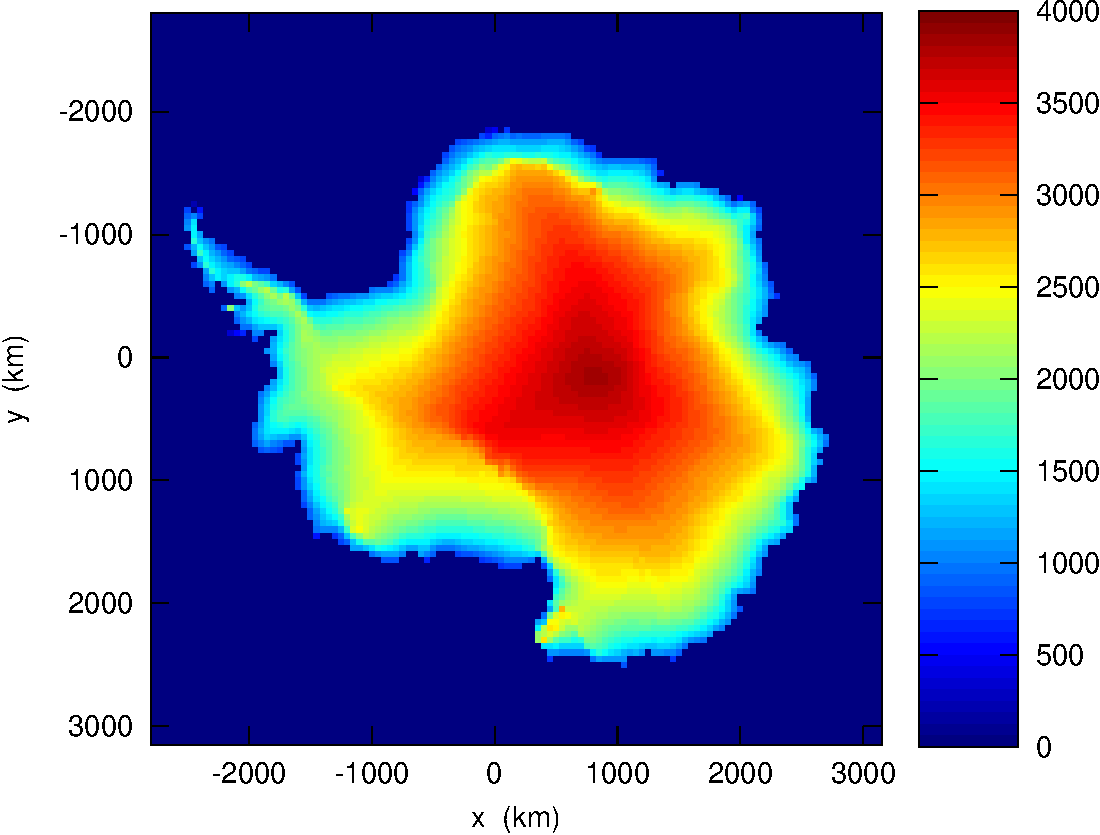
\includegraphics[height=1.75in]{antfinal}
\end{column}
\end{columns}
\end{frame}


\begin{frame}{final comments on SIA: origin and rigor}

where does the ``shallow ice approximation'' come from?:
\bigskip

\begin{itemize}
\item historically, Fowler and Larson (1978), Morland and Johnson (1980), and Hutter (1983) \dots thus recent
\item logically, by a ``small-parameter argument'', based on a small depth-to-width ratio, from the more complete Stokes model for slow ice flow
\item more precisely, by using the small aspect ratio \, $\eps = [H]/[L]$ \, of ice sheets to scale the Stokes model to see which terms make small contributions
\end{itemize}
\end{frame}